
        \documentclass[12p]{article}
        \usepackage[margin=1in, left=1.5in, includefoot]{geometry}
        \usepackage{longtable, tabu}
        \usepackage[table, dvipsnames]{xcolor}
        \usepackage{array,booktabs}
        \usepackage{color}
        \usepackage{indentfirst}
        \usepackage{graphicx}
        \usepackage{float}
        \usepackage[utf8]{inputenc}
        \usepackage{listings}
        \usepackage{url}
        
        \definecolor{ferrarired}{rgb}{1.0, 0.11, 0.0}
        \definecolor{orange(colorwheel)}{rgb}{1.0, 0.5, 0.0}
        \definecolor{deepskyblue}{rgb}{0.0, 0.75, 1.0}
        \definecolor{grannysmithapple}{rgb}{0.66, 0.89, 0.63}
        \definecolor{gray(x11gray)}{rgb}{0.75, 0.75, 0.75}
        \definecolor{amber}{rgb}{1.0, 0.75, 0.0}
        
        \newcommand{\icon}[1]{\includegraphics[height=12pt]{#1}}
        \setlength{\arrayrulewidth}{0.3mm}
\setlength{\tabcolsep}{18pt}
\renewcommand{\arraystretch}{1.5}
\setlength{\parindent}{1em}
\begin{document}
\begin{titlepage}
\begin{center}
\line(1,0){320}\\
[0.25in]
\huge{\bfseries Android Analysis Report}
\line(1,0){320}\\
[0.5in]
\begin{figure}[H]
	\centering
	
\includegraphics[scale=0.5]{/home/miki/Documents/GITHUB/AndroidPermissions/python/vulns/report_icons/logo.png}
\end{figure}
\textsl{\LARGE Insecure Bank}\\
\textsf{\LARGE com.insecurebnk}\\
[2.5in]
\end{center}
\begin{flushright}
\textbf{\large Date 2018-06-13}
\end{flushright}
\end{titlepage}
\tableofcontents
\thispagestyle{empty}
\cleardoublepage
\setcounter{page}{1}
\section{FINDINGS SUMMARY}\label{sec:summary}
	\begin{longtable}{p{0.5cm} p{10cm} p{1.5cm}}
	\rowcolor{grannysmithapple!70} Index & Title & Impact \\
	A1&JavascriptInterfaceAnalyser& \color{ferrarired}\textbf{High} \\
\hline\\	A2&MixedContentAnalyser& \color{ferrarired}\textbf{High} \\
\hline\\	A3&Non-random XOR& \color{ferrarired}\textbf{High} \\
\hline\\	A4&testing& \color{amber}\textbf{Low} \\
\hline\\	A5&Electronic Codebook \newline (ECB) used for encryption& \color{ferrarired}\textbf{High} \\
\hline\\	A6&Application Data can be Backed up& \color{orange(colorwheel)}\textbf{Medium} \\
\hline\\	A7&Activity \newline (com. android. insecurebankv2. PostLogin) is not Protected. [android:exported=true]& \color{ferrarired}\textbf{High} \\
\hline\\	A8&Activity \newline (com. android. insecurebankv2. DoTransfer) is not Protected. [android:exported=true]& \color{ferrarired}\textbf{High} \\
\hline\\	A9&Activity \newline (com. android. insecurebankv2. ViewStatement) is not Protected. [android:exported=true]& \color{ferrarired}\textbf{High} \\
\hline\\	A10&Content Provider \newline (com. android. insecurebankv2. TrackUserContentProvider) is not Protected. [android:exported=true]& \color{ferrarired}\textbf{High} \\
\hline\\	A11&Broadcast Receiver \newline (com. android. insecurebankv2. MyBroadCastReceiver) is not Protected. [android:exported=true]& \color{ferrarired}\textbf{High} \\
\hline\\	A12&Activity \newline (com. android. insecurebankv2. ChangePassword) is not Protected. [android:exported=true]& \color{ferrarired}\textbf{High} \\
\hline\\	A13&& \color{amber}\textbf{Low} \\
\hline\\	\end{longtable}
\cleardoublepage
\section{DETAILED FINDINGS}
\subsection{A1: JavascriptInterfaceAnalyser}
\subsubsection*{\protect\icon{/home/miki/Documents/GITHUB/AndroidPermissions/python/vulns/report_icons/basic_sheet.png} Description}

\subsubsection*{\protect\icon{/home/miki/Documents/GITHUB/AndroidPermissions/python/vulns/report_icons/basic_magnifier.png} Evidence}
\path{/home/miki/Documents/GITHUB/AndroidPermissions/apks/test_apks/insecurebank/app/smali/com/google/android/gms/internal/zzig.smali addJavascriptInterface}

\subsubsection*{\protect\icon{/home/miki/Documents/GITHUB/AndroidPermissions/python/vulns/report_icons/basic_todo.png} Recommendation}

\subsection{A2: MixedContentAnalyser}
\subsubsection*{\protect\icon{/home/miki/Documents/GITHUB/AndroidPermissions/python/vulns/report_icons/basic_sheet.png} Description}

\subsubsection*{\protect\icon{/home/miki/Documents/GITHUB/AndroidPermissions/python/vulns/report_icons/basic_magnifier.png} Evidence}
\path{/home/miki/Documents/GITHUB/AndroidPermissions/apks/test_apks/insecurebank/app/smali/com/google/android/gms/internal/zzig.smali}

\subsubsection*{\protect\icon{/home/miki/Documents/GITHUB/AndroidPermissions/python/vulns/report_icons/basic_todo.png} Recommendation}

\subsection{A3: Non-random XOR}
\subsubsection*{\protect\icon{/home/miki/Documents/GITHUB/AndroidPermissions/python/vulns/report_icons/basic_sheet.png} Description}
Test description
\subsubsection*{\protect\icon{/home/miki/Documents/GITHUB/AndroidPermissions/python/vulns/report_icons/basic_magnifier.png} Evidence}
\path{/app/smali/com/google/android/gms/internal/zzai$zzk.smali xor-int/lit8 v2, v2, -0x1}

\path{/app/smali/com/google/android/gms/internal/zzai$zzj.smali xor-int/lit8 v2, v2, -0x1}

\path{/app/smali/android/support/v4/util/LongSparseArray.smali xor-int/lit8 v0, v0, -0x1}

\path{/app/smali/com/google/android/gms/internal/zzrj.smali xor-int/lit8 v0, v0, -0x1}

\path{/app/smali/com/google/android/gms/internal/zzai$zze.smali xor-int/lit8 v1, v1, -0x1}

\path{/app/smali/com/google/android/gms/internal/zzai$zzd.smali xor-int/lit8 v1, v1, -0x1}

\path{/app/smali/com/google/android/gms/internal/zzai$zzg.smali xor-int/lit8 v2, v2, -0x1}

\path{/app/smali/com/google/android/gms/internal/zzai$zzi.smali xor-int/lit8 v2, v2, -0x1}

\path{/app/smali/com/google/android/gms/internal/zzai$zzb.smali xor-int/lit8 v2, v2, -0x1}

\path{/app/smali/com/google/android/gms/internal/zzai$zzl.smali xor-int/lit8 v2, v2, -0x1}


\textit{snip}
\newline \textsl{For the full list view \path{/home/miki/Documents/GITHUB/AndroidPermissions/apks/test_apks/insecurebank/report}}
\subsubsection*{\protect\icon{/home/miki/Documents/GITHUB/AndroidPermissions/python/vulns/report_icons/basic_todo.png} Recommendation}
Test recommendation
\subsection{A4: testing}
\subsubsection*{\protect\icon{/home/miki/Documents/GITHUB/AndroidPermissions/python/vulns/report_icons/basic_sheet.png} Description}

\subsubsection*{\protect\icon{/home/miki/Documents/GITHUB/AndroidPermissions/python/vulns/report_icons/basic_magnifier.png} Evidence}
\path{/home/miki/Documents/GITHUB/AndroidPermissions/apks/test_apks/insecurebank/app/smali/android/support/v4/text/ICUCompatIcs.smali
Landroid/util/Log -> w(Ljava/lang/String;Ljava/lang/Throwable;)}

\path{/home/miki/Documents/GITHUB/AndroidPermissions/apks/test_apks/insecurebank/app/smali/android/support/v4/text/ICUCompatIcs.smali
Landroid/util/Log -> w(Ljava/lang/String;Ljava/lang/Throwable;)}

\path{/home/miki/Documents/GITHUB/AndroidPermissions/apks/test_apks/insecurebank/app/smali/android/support/v4/text/ICUCompatIcs.smali
Landroid/util/Log -> w(Ljava/lang/String;Ljava/lang/Throwable;)}

\path{/home/miki/Documents/GITHUB/AndroidPermissions/apks/test_apks/insecurebank/app/smali/android/support/v4/text/ICUCompatIcs.smali
Landroid/util/Log -> w(Ljava/lang/String;Ljava/lang/Throwable;)}

\path{/home/miki/Documents/GITHUB/AndroidPermissions/apks/test_apks/insecurebank/app/smali/android/support/v4/text/ICUCompatIcs.smali
Landroid/util/Log -> w(Ljava/lang/String;Ljava/lang/Throwable;)}

\path{/home/miki/Documents/GITHUB/AndroidPermissions/apks/test_apks/insecurebank/app/smali/android/support/v4/print/PrintHelperKitkat$1.smali
Landroid/util/Log -> e(Ljava/lang/String;Ljava/lang/String;Ljava/lang/Throwable;)}

\path{/home/miki/Documents/GITHUB/AndroidPermissions/apks/test_apks/insecurebank/app/smali/android/support/v4/print/PrintHelperKitkat.smali
Landroid/util/Log -> w(Ljava/lang/String;Ljava/lang/String;Ljava/lang/Throwable;)}

\path{/home/miki/Documents/GITHUB/AndroidPermissions/apks/test_apks/insecurebank/app/smali/android/support/v4/print/PrintHelperKitkat.smali
Landroid/util/Log -> w(Ljava/lang/String;Ljava/lang/String;Ljava/lang/Throwable;)}

\path{/home/miki/Documents/GITHUB/AndroidPermissions/apks/test_apks/insecurebank/app/smali/android/support/v4/print/PrintHelperKitkat$2.smali
Landroid/util/Log -> e(Ljava/lang/String;Ljava/lang/String;Ljava/lang/Throwable;)}

\path{/home/miki/Documents/GITHUB/AndroidPermissions/apks/test_apks/insecurebank/app/smali/android/support/v4/util/AtomicFile.smali
Landroid/util/Log -> w(Ljava/lang/String;Ljava/lang/String;Ljava/lang/Throwable;)}


\textit{snip}
\newline \textsl{For the full list view \path{/home/miki/Documents/GITHUB/AndroidPermissions/apks/test_apks/insecurebank/report}}
\subsubsection*{\protect\icon{/home/miki/Documents/GITHUB/AndroidPermissions/python/vulns/report_icons/basic_todo.png} Recommendation}

\subsection{A5: Electronic Codebook (ECB) used for encryption}
\subsubsection*{\protect\icon{/home/miki/Documents/GITHUB/AndroidPermissions/python/vulns/report_icons/basic_sheet.png} Description}

            Using the same encryption key, in ECB mode data blocks are enciphered individually 
            from each other and cause identical message blocks to be transformed to identical ciphertext 
            blocks. The independency of encrypted blocks also implies that the malicious substitution of a 
            block has no impact on adjacent blocks. As a consequence, data patterns are not well hidden and 
            message confidentiality may be compromised.
            
            On Android, the Cipher API provides access to implementations of cryptographic schemes
            for the encryption and decryption of arbitrary data. To request an instance of a particular cipher,
            an application has to invoke the method getInstance, passing a suitable transformation string as
            parameter. Typically, this value is composed of the desired algorithm name, a mode of operation,
            and the padding scheme to apply. For example, to request an object instance that provides AES in
            ECB mode with PKCS5 padding, the transformation AES/ECB/PKCS5Padding has to be specified.
            
            While it is indispensable to declare the algorithm to use, explicitly setting the mode and
            padding may be omitted. To fill the gap, the underlying Cryptographic Service Provider (CSP)
            relies on predefined values that do not necessarily reflect the recommended practice. Precisely, if
            the transformation indicates no operation mode, ECB mode is put in place. Moreover, the initially
            described problem with ECB is not limited to a specific cipher, such as AES but affects all symmetric
            block ciphers. Stream ciphers and asymmetric cryptosystems are not concerned since they
            do not involve an operation mode to repeatedly encipher blocks of contiguous data.
        
\subsubsection*{\protect\icon{/home/miki/Documents/GITHUB/AndroidPermissions/python/vulns/report_icons/basic_magnifier.png} Evidence}
\path{/home/miki/Documents/GITHUB/AndroidPermissions/apks/test_apks/insecurebank/app/smali/com/android/insecurebankv2/CryptoClass.smali}

\path{/home/miki/Documents/GITHUB/AndroidPermissions/apks/test_apks/insecurebank/app/smali/com/android/insecurebankv2/CryptoClass.smali}

\path{/home/miki/Documents/GITHUB/AndroidPermissions/apks/test_apks/insecurebank/app/smali/com/google/android/gms/internal/zzar.smali}

\subsubsection*{\protect\icon{/home/miki/Documents/GITHUB/AndroidPermissions/python/vulns/report_icons/basic_todo.png} Recommendation}
It is recommended not to use ECB for encryption. Use an asymmetric encryption algorithm instead
\subsection{A6: Application Data can be Backed up}
\subsubsection*{\protect\icon{/home/miki/Documents/GITHUB/AndroidPermissions/python/vulns/report_icons/basic_sheet.png} Description}
This flag allows anyone to backup your application data via adb. It allows users who have enabled USB debugging to copy application data off of the device.
\subsubsection*{\protect\icon{/home/miki/Documents/GITHUB/AndroidPermissions/python/vulns/report_icons/basic_todo.png} Recommendation}
android:allowBackup = False
\subsection{A7: Activity (com. android. insecurebankv2. PostLogin) is not Protected. [android:exported=true]}
\subsubsection*{\protect\icon{/home/miki/Documents/GITHUB/AndroidPermissions/python/vulns/report_icons/basic_sheet.png} Description}
A Activity is found to be shared with other apps on the device therefore leaving it accessible to any other application on the device.
\subsubsection*{\protect\icon{/home/miki/Documents/GITHUB/AndroidPermissions/python/vulns/report_icons/basic_todo.png} Recommendation}
It is recommended to set the protection level to signature, so only applications signed with the same certificate can obtain the permission.
\subsection{A8: Activity (com. android. insecurebankv2. DoTransfer) is not Protected. [android:exported=true]}
\subsubsection*{\protect\icon{/home/miki/Documents/GITHUB/AndroidPermissions/python/vulns/report_icons/basic_sheet.png} Description}
A Activity is found to be shared with other apps on the device therefore leaving it accessible to any other application on the device.
\subsubsection*{\protect\icon{/home/miki/Documents/GITHUB/AndroidPermissions/python/vulns/report_icons/basic_todo.png} Recommendation}
It is recommended to set the protection level to signature, so only applications signed with the same certificate can obtain the permission.
\subsection{A9: Activity (com. android. insecurebankv2. ViewStatement) is not Protected. [android:exported=true]}
\subsubsection*{\protect\icon{/home/miki/Documents/GITHUB/AndroidPermissions/python/vulns/report_icons/basic_sheet.png} Description}
A Activity is found to be shared with other apps on the device therefore leaving it accessible to any other application on the device.
\subsubsection*{\protect\icon{/home/miki/Documents/GITHUB/AndroidPermissions/python/vulns/report_icons/basic_todo.png} Recommendation}
It is recommended to set the protection level to signature, so only applications signed with the same certificate can obtain the permission.
\subsection{A10: Content Provider (com. android. insecurebankv2. TrackUserContentProvider) is not Protected. [android:exported=true]}
\subsubsection*{\protect\icon{/home/miki/Documents/GITHUB/AndroidPermissions/python/vulns/report_icons/basic_sheet.png} Description}
A Content Provider is found to be shared with other apps on the device therefore leaving it accessible to any other application on the device.
\subsubsection*{\protect\icon{/home/miki/Documents/GITHUB/AndroidPermissions/python/vulns/report_icons/basic_todo.png} Recommendation}
It is recommended to set the protection level to signature, so only applications signed with the same certificate can obtain the permission.
\subsection{A11: Broadcast Receiver (com. android. insecurebankv2. MyBroadCastReceiver) is not Protected. [android:exported=true]}
\subsubsection*{\protect\icon{/home/miki/Documents/GITHUB/AndroidPermissions/python/vulns/report_icons/basic_sheet.png} Description}
A Broadcast Receiver is found to be shared with other apps on the device therefore leaving it accessible to any other application on the device.
\subsubsection*{\protect\icon{/home/miki/Documents/GITHUB/AndroidPermissions/python/vulns/report_icons/basic_todo.png} Recommendation}
It is recommended to set the protection level to signature, so only applications signed with the same certificate can obtain the permission.
\subsection{A12: Activity (com. android. insecurebankv2. ChangePassword) is not Protected. [android:exported=true]}
\subsubsection*{\protect\icon{/home/miki/Documents/GITHUB/AndroidPermissions/python/vulns/report_icons/basic_sheet.png} Description}
A Activity is found to be shared with other apps on the device therefore leaving it accessible to any other application on the device.
\subsubsection*{\protect\icon{/home/miki/Documents/GITHUB/AndroidPermissions/python/vulns/report_icons/basic_todo.png} Recommendation}
It is recommended to set the protection level to signature, so only applications signed with the same certificate can obtain the permission.
\subsection{A13: }
\subsubsection*{\protect\icon{/home/miki/Documents/GITHUB/AndroidPermissions/python/vulns/report_icons/basic_sheet.png} Description}

\subsubsection*{\protect\icon{/home/miki/Documents/GITHUB/AndroidPermissions/python/vulns/report_icons/basic_magnifier.png} Evidence}
\path{/home/miki/Documents/GITHUB/AndroidPermissions/apks/test_apks/insecurebank/app/smali/android/support/v4/text/ICUCompatIcs.smali forName}

\path{/home/miki/Documents/GITHUB/AndroidPermissions/apks/test_apks/insecurebank/app/smali/android/support/v4/text/ICUCompatIcs.smali invoke}

\path{/home/miki/Documents/GITHUB/AndroidPermissions/apks/test_apks/insecurebank/app/smali/android/support/v4/text/ICUCompatIcs.smali invoke}

\path{/home/miki/Documents/GITHUB/AndroidPermissions/apks/test_apks/insecurebank/app/smali/android/support/v4/util/MapCollections.smali getComponentType}

\path{/home/miki/Documents/GITHUB/AndroidPermissions/apks/test_apks/insecurebank/app/smali/android/support/v4/app/NotificationCompatJellybean.smali forName}

\path{/home/miki/Documents/GITHUB/AndroidPermissions/apks/test_apks/insecurebank/app/smali/android/support/v4/app/ActionBarDrawerToggleHoneycomb.smali invoke}

\path{/home/miki/Documents/GITHUB/AndroidPermissions/apks/test_apks/insecurebank/app/smali/android/support/v4/app/ActionBarDrawerToggleHoneycomb.smali invoke}

\path{/home/miki/Documents/GITHUB/AndroidPermissions/apks/test_apks/insecurebank/app/smali/android/support/v4/media/routing/MediaRouterJellybean$GetDefaultRouteWorkaround.smali invoke}

\path{/home/miki/Documents/GITHUB/AndroidPermissions/apks/test_apks/insecurebank/app/smali/android/support/v4/media/routing/MediaRouterJellybeanMr1$IsConnectingWorkaround.smali invoke}

\path{/home/miki/Documents/GITHUB/AndroidPermissions/apks/test_apks/insecurebank/app/smali/android/support/v4/media/routing/MediaRouterJellybeanMr1$ActiveScanWorkaround.smali invoke}


\textit{snip}
\newline \textsl{For the full list view \path{/home/miki/Documents/GITHUB/AndroidPermissions/apks/test_apks/insecurebank/report}}
\subsubsection*{\protect\icon{/home/miki/Documents/GITHUB/AndroidPermissions/python/vulns/report_icons/basic_todo.png} Recommendation}

\begin{figure}[H]
	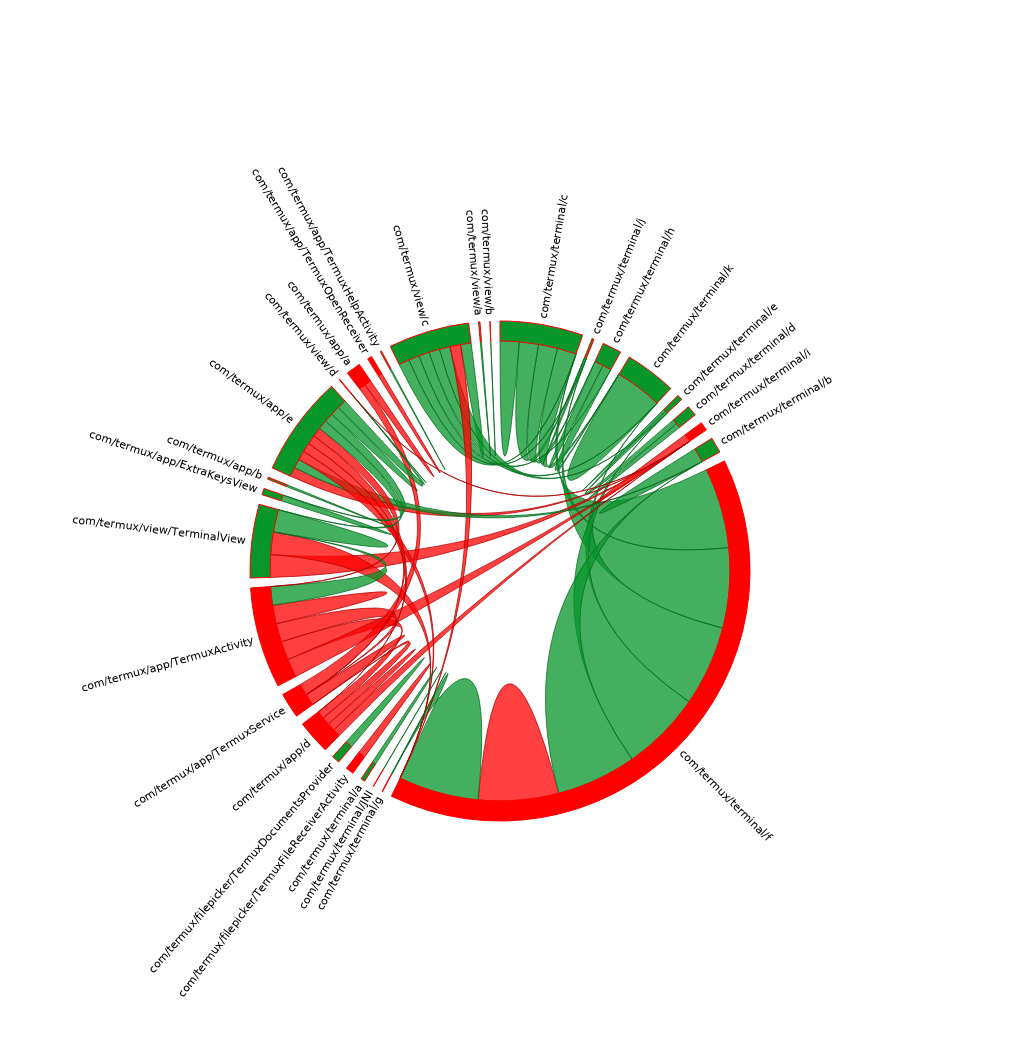
\includegraphics[scale=0.4]{/home/miki/Documents/GITHUB/AndroidPermissions/apks/test_apks/insecurebank/report/chord_diagram.png}\end{figure}\begin{figure}[H]
	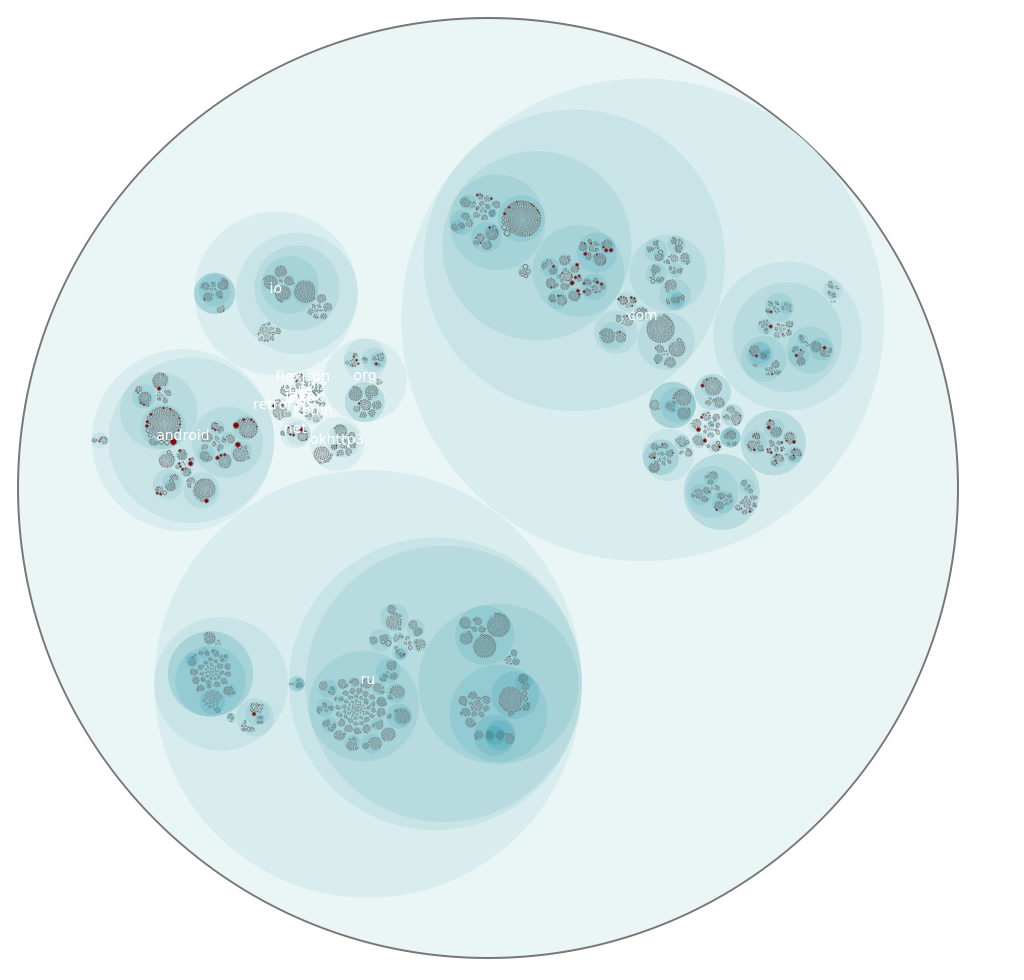
\includegraphics[scale=0.5]{/home/miki/Documents/GITHUB/AndroidPermissions/apks/test_apks/insecurebank/report/hotspot.png}\end{figure}\begin{longtable}{p{0.5cm} p{10cm}}
\rowcolor{red} Index & Class \\
1 & \path{/home/miki/Documents/GITHUB/AndroidPermissions/apks/playstore_apps/com_termux/app/smali/com/termux/app/TermuxActivity$1.smali} \\
2 & \path{/home/miki/Documents/GITHUB/AndroidPermissions/apks/playstore_apps/com_termux/app/smali/com/termux/app/TermuxActivity$1.smali} \\
3 & \path{/home/miki/Documents/GITHUB/AndroidPermissions/apks/playstore_apps/com_termux/app/smali/com/termux/app/TermuxActivity$1.smali} \\
4 & \path{/home/miki/Documents/GITHUB/AndroidPermissions/apks/playstore_apps/com_termux/app/smali/com/termux/app/TermuxActivity$1.smali} \\
5 & \path{/home/miki/Documents/GITHUB/AndroidPermissions/apks/playstore_apps/com_termux/app/smali/com/termux/app/TermuxActivity$1.smali} \\
6 & \path{/home/miki/Documents/GITHUB/AndroidPermissions/apks/playstore_apps/com_termux/app/smali/com/termux/app/TermuxActivity$1.smali} \\
7 & \path{/home/miki/Documents/GITHUB/AndroidPermissions/apks/playstore_apps/com_termux/app/smali/com/termux/app/TermuxActivity$1.smali} \\
	\end{longtable}
\end{document}
